%        روش اجرا.: 2 بار F1 ، 2 بار  F11(به منظور تولید مراجع) ، دوبار Ctrl+Alt+I (به منظور تولید نمایه) و دو بار F1 -------> مشاهده Pdf
%%%%%%%%%%%%%%%%%%%%%%%%%%%%%%%%%%%%%%%%%%%%%%%%%%%%%%
%   TeXstudio as your IDE
%%  برای compile در TeXstudio تنها کافی است منوی Options->Configure TeXstudio را زده و در پنجره Configure TeXstudio در بخش Build گزینه Default Compiler را به XeLaTeX تغییر دهید. سند شما به راحتی compile خواهد شد.
%   F1 & F5 : Build & view
%   F6      : Compile
%   F7      : View
%   --------------
%%%%%%%%%%%%%%%%%%%%%%%%%%%%%%%%%%%%%%%%%%%%%%%%%%%%%%
%%% !TEX TS-program = XeLaTeX
	\documentclass[oneside,msc,12pt]{LaTeXClass}
%       فایل commands.tex را حتماً به دقت مطالعه کنید؛ چون دستورات مربوط به فراخوانی بسته زی‌پرشین 
%       و دیگر بسته‌ها و ... در این فایل قرار دارد و بهتر است که با نحوه استفاده از آنها آشنا شوید. توجه شود برای نسخه نهایی سند حتماً hyperref را غیرفعال کنید.
	% در این فایل، دستورها و تنظیمات مورد نیاز، آورده شده است.
%-------------------------------------------------------------------------------------------------------------------
% در ورژن جدید زی‌پرشین برای تایپ متن‌های ریاضی، این سه بسته، حتماً باید فراخوانی شود.
\setcounter{secnumdepth}{3}
\setcounter{tocdepth}{3}
\usepackage{multicol}
\usepackage{shapepar}

\usepackage{amsthm,amssymb,amsmath,amsfonts}
% بسته‌ای برای تنطیم حاشیه‌های بالا، پایین، چپ و راست صفحه
\usepackage[top=30mm, bottom=30mm, left=25mm, right=30mm]{geometry}
% بسته‌‌ای برای ظاهر شدن شکل‌ها و تصاویر متن
\usepackage{graphicx}
\usepackage{color}
\usepackage{xcolor}
%بسته‌ای برای تنظیم فاصله عمودی خط‌های متن
\usepackage{setspace}
\usepackage{titletoc}
\usepackage{tocloft}
%با فعال کردن بسته زیر فوت‌نوت‌ها در هر صفحه ریست می‌شوند. حالت پیش‌فرض آن ریست شدن در هر فصل می‌باشد.
%\usepackage[perpage]{footmisc}

%\usepackage{titlesec}
% بسته‌ و دستوراتی برای ایجاد لینک‌های رنگی با امکان جهش
\usepackage[pagebackref=false,colorlinks,linkcolor=blue,citecolor=red]{hyperref}
\usepackage[nameinlink]{cleveref}%capitalize,,noabbrev
 \AtBeginDocument{%
    \crefname{equation}{برابری}{equations}%
    \crefname{chapter}{فصل}{chapters}%
    \crefname{section}{بخش}{sections}%
    \crefname{appendix}{پیوست}{appendices}%
    \crefname{enumi}{مورد}{items}%
    \crefname{footnote}{زیرنویس}{footnotes}%
    \crefname{figure}{شکل}{figures}%
    \crefname{table}{جدول}{tables}%
    \crefname{theorem}{قضیه}{theorems}%
    \crefname{lemma}{لم}{lemmas}%
    \crefname{corollary}{نتیجه}{corollaries}%
    \crefname{proposition}{گزاره}{propositions}%
    \crefname{definition}{تعریف}{definitions}%
    \crefname{result}{نتیجه}{results}%
    \crefname{example}{مثال}{examples}%
    \crefname{remark}{نکته}{remarks}%
    \crefname{note}{یادداشت}{notes}%
}
\usepackage{enumitem}
\usepackage{cleveref}
\usepackage{tikz,lmodern,amssymb}
\tcbuselibrary{skins,breakable}

% چنانچه قصد پرینت گرفتن نوشته خود را دارید، خط بالا را غیرفعال و  از دستور زیر استفاده کنید چون در صورت استفاده از دستور زیر‌‌، 
% لینک‌ها به رنگ سیاه ظاهر خواهند شد که برای پرینت گرفتن، مناسب‌تر است
%\usepackage[pagebackref=false]{hyperref}
% بسته‌ لازم برای تنظیم سربرگ‌ها
\usepackage{fancyhdr}
% بسته‌ای برای ظاهر شدن «مراجع»  در فهرست مطالب
\usepackage[nottoc]{tocbibind}
% دستورات مربوط به ایجاد نمایه
\usepackage{makeidx,multicol}
\setlength{\columnsep}{1.5cm}

%%%%%%%%%%%%%%%%%%%%%%%%%%
\usepackage{verbatim}
\makeindex
\usepackage{sectsty}

% فراخوانی بسته زی‌پرشین و تعریف قلم فارسی و انگلیسی
\usepackage{xepersian}%[extrafootnotefeatures]
\SepMark{-}
%حتماً از تک لایو 2014 استفاده کنید.
\settextfont[Scale=1.2]{IRNazanin}
\setlatintextfont{Times New Roman}
\renewcommand{\labelitemi}{$\bullet$}
%%%%%%%%%%%%%%%%%%%%%%%%%%
% چنانچه می‌خواهید اعداد در فرمول‌ها، انگلیسی باشد، خط زیر را غیرفعال کنید.
%در غیر اینصورت حتماً فونت PGaramond را نصب کنید.
\setdigitfont[Scale=1.1]{Yas}%%Yas
%%%%%%%%%%%%%%%%%%%%%%%%%%
% تعریف قلم‌های فارسی اضافی برای استفاده در بعضی از قسمت‌های متن
\defpersianfont\nastaliq[Scale=2]{IranNastaliq}
\defpersianfont\chapternumber[Scale=3]{B Nazanin}
%\chapterfont{\centering}%
%%%%%%%%%%%%%%%%%%%%%%%%%%
% دستوری برای تغییر نام کلمه «اثبات» به «برهان»
\renewcommand\proofname{\textbf{برهان}}

% دستوری برای تغییر نام کلمه «کتاب‌نامه» به «منابع و مراجع«
\renewcommand{\bibname}{منابع و مراجع}


% Headings for every page of ToC, LoF and Lot
\setlength{\cftbeforetoctitleskip}{-1.2em}
\setlength{\cftbeforelottitleskip}{-1.2em}
\setlength{\cftbeforeloftitleskip}{-1.2em}
\setlength{\cftaftertoctitleskip}{-1em}
\setlength{\cftafterlottitleskip}{-1em}
\setlength{\cftafterloftitleskip}{-1em}
%%\makeatletter
%%%%\renewcommand{\l@chapter}{\@dottedtocline{1}{1em\bfseries}{1em}}
%%%%\renewcommand{\l@section}{\@dottedtocline{2}{2em}{2em}}
%%%%\renewcommand{\l@subsection}{\@dottedtocline{3}{3em}{3em}}
%%%%\renewcommand{\l@subsubsection}{\@dottedtocline{4}{4em}{4em}}
%%%%\makeatother


\newcommand\tocheading{\par عنوان\hfill صفحه \par}
\newcommand\lofheading{\hspace*{.5cm}\figurename\hfill صفحه \par}
\newcommand\lotheading{\hspace*{.5cm}\tablename\hfill صفحه \par}

\renewcommand{\cftchapleader}{\cftdotfill{\cftdotsep}}
\renewcommand{\cfttoctitlefont}{\hspace*{\fill}\LARGE\bfseries}%\Large
\renewcommand{\cftaftertoctitle}{\hspace*{\fill}}
\renewcommand{\cftlottitlefont}{\hspace*{\fill}\LARGE\bfseries}%\Large
\renewcommand{\cftafterlottitle}{\hspace*{\fill}}
\renewcommand{\cftloftitlefont}{\hspace*{\fill}\LARGE\bfseries}
\renewcommand{\cftafterloftitle}{\hspace*{\fill}}

%%%%%%%%%%%%%%%%%%%%%%%%%%
% تعریف و نحوه ظاهر شدن عنوان قضیه‌ها، تعریف‌ها، مثال‌ها و ...
%برای شماره گذاری سه تایی قضیه ها

\makeatletter
% restore footnote and LTRfootnote internals to those in normal page, not minipage
\def\tcb@restore@footnote{%
	\def\@mpfn{footnote}%
	\def\thempfn{\arabic{footnote}}%
	\let\@footnotetext\tcb@footnote@collect
	\let\@LTRfootnotetext\tcb@LTRfootnote@collect
}
% collect footnote text
\long\def\tcb@footnote@collect#1{%
	% expand \@thefnmark before appending before app to \tcb@footnote@acc
	\expandafter\gappto\expandafter\tcb@footnote@acc\expandafter{%
		\expandafter\footnotetext\expandafter[\@thefnmark]{#1}%
	}%
}
% collect LTRfootnote text
\long\def\tcb@LTRfootnote@collect#1{%
	% expand \@thefnmark before appending before app to \tcb@footnote@acc
	\expandafter\gappto\expandafter\tcb@footnote@acc\expandafter{%
		\expandafter\LTRfootnotetext\expandafter[\@thefnmark]{#1}%
	}%
}
\def\tcb@footnote@use{%
	\tcb@footnote@acc
	\global\let\tcb@footnote@acc\@empty
}
\global\let\tcb@footnote@acc\@empty
\tcbset{
	% restore for every box
	every box/.style={%
		before upper pre=\tcb@restore@footnote
	},
	% use for layer 1 boxes only
	every box on layer 1/.append style={%
		after app=\tcb@footnote@use
	}%
}
\makeatother


\newtcolorbox[auto counter,number within=section,
number freestyle={(\noexpand\arabic{\tcbcounter}-\thesection)},
]{phbox}[2][]{%
	colback=yellow!15!white,colframe=blue!75!black,fonttitle=\bfseries,
	title=تمرین~\thetcbcounter: #2,#1}

\newtcolorbox[auto counter,number within=section,
number freestyle={(\noexpand\arabic{\tcbcounter}-\thesection)},
]{phboxr}[2][]{%
	colback=yellow!15!white,colframe=red!75!black,fonttitle=\bfseries,
	title=تمرین~\thetcbcounter: #2,#1}


\theoremstyle{definition}
\newtheorem{definition}{تعریف}[section]
\newtheorem{remark}[definition]{نکته}
\newtheorem{note}[definition]{یادداشت}
\newtheorem{example}[definition]{نمونه}
\newtheorem{question}[definition]{سوال}
\newtheorem{remember}[definition]{یاداوری}
\theoremstyle{theorem}
\newtheorem{theorem}[definition]{قضیه}
\newtheorem{lemma}[definition]{لم}
\newtheorem{proposition}[definition]{گزاره}
\newtheorem{corollary}[definition]{نتیجه}


%%%%%%%%%%%%%%%%%%%%%%%%
%%%%%%%%%%%%%%%%%%%
%%% برای شماره گذاری چهارتایی قضیه ها و ...
%%\newtheorem{definition1}[subsubsection]{تعریف}
%%\newtheorem{theorem1}[subsubsection]{قضیه}
%%\newtheorem{lemma1}[subsubsection]{لم}
%%\newtheorem{proposition1}[subsubsection]{گزاره}
%%\newtheorem{corollary1}[subsubsection]{نتیجه}
%%\newtheorem{remark1}[subsubsection]{نکته}
%%\newtheorem{example1}[subsubsection]{مثال}
%%\newtheorem{question1}[subsubsection]{سوال}

%%%%%%%%%%%%%%%%%%%%%%%%%%%%

% دستورهایی برای سفارشی کردن صفحات اول فصل‌ها
\makeatletter
\newcommand\mycustomraggedright{%
 \if@RTL\raggedleft%
 \else\raggedright%
 \fi}
\def\@makechapterhead#1{%
\thispagestyle{style1}
\vspace*{20\p@}%
{\parindent \z@ \mycustomraggedright
\ifnum \c@secnumdepth >\m@ne
\if@mainmatter

\bfseries{\Huge \@chapapp}\small\space {\chapternumber\thechapter}
\par\nobreak
\vskip 0\p@
\fi
\fi
\interlinepenalty\@M 
\Huge \bfseries #1\par\nobreak
\vskip 120\p@

}

%\thispagestyle{empty}
\newpage}
\bidi@patchcmd{\@makechapterhead}{\thechapter}{\tartibi{chapter}}{}{}
\bidi@patchcmd{\chaptermark}{\thechapter}{\tartibi{chapter}}{}{}
\makeatother

\pagestyle{fancy}
\renewcommand{\chaptermark}[1]{\markboth{\chaptername~\tartibi{chapter}: #1}{}}

\fancypagestyle{style1}{
\fancyhf{} 
\fancyfoot[c]{\thepage}
\fancyhead[R]{\leftmark}%
\renewcommand{\headrulewidth}{1.2pt}
}


\fancypagestyle{style2}{
\fancyhf{}
\fancyhead[R]{چکیده}
\fancyfoot[C]{\thepage{}}
\renewcommand{\headrulewidth}{1.2pt}
}

\fancypagestyle{style3}{%
  \fancyhf{}%
  \fancyhead[R]{فهرست نمادها}
  \fancyfoot[C]{\thepage}%
  \renewcommand{\headrulewidth}{1.2pt}%
}

\fancypagestyle{style4}{%
  \fancyhf{}%
  \fancyhead[R]{فهرست جداول}
  \fancyfoot[C]{\thepage}%
  \renewcommand{\headrulewidth}{1.2pt}%
}

\fancypagestyle{style5}{%
  \fancyhf{}%
  \fancyhead[R]{فهرست اشکال}
  \fancyfoot[C]{\thepage}%
  \renewcommand{\headrulewidth}{1.2pt}%
}

\fancypagestyle{style6}{%
  \fancyhf{}%
  \fancyhead[R]{فهرست مطالب}
  \fancyfoot[C]{\thepage}%
  \renewcommand{\headrulewidth}{1.2pt}%
}

\fancypagestyle{style7}{%
  \fancyhf{}%
  \fancyhead[R]{نمایه}
  \fancyfoot[C]{\thepage}%
  \renewcommand{\headrulewidth}{1.2pt}%
}

\fancypagestyle{style8}{%
  \fancyhf{}%
  \fancyhead[R]{منابع و مراجع}
  \fancyfoot[C]{\thepage}%
  \renewcommand{\headrulewidth}{1.2pt}%
}
\fancypagestyle{style9}{%
  \fancyhf{}%
  \fancyhead[R]{واژه‌نامه‌ی فارسی به انگلیسی}
  \fancyfoot[C]{\thepage}%
  \renewcommand{\headrulewidth}{1.2pt}%
}
%


%دستور حذف نام لیست تصاویر و لیست جداول از فهرست مطالب
\newcommand*{\BeginNoToc}{%
  \addtocontents{toc}{%
    \edef\protect\SavedTocDepth{\protect\the\protect\value{tocdepth}}%
  }%
  \addtocontents{toc}{%
    \protect\setcounter{tocdepth}{-10}%
  }%
}
\newcommand*{\EndNoToc}{%
  \addtocontents{toc}{%
    \protect\setcounter{tocdepth}{\protect\SavedTocDepth}%
  }%
}
\newcounter{savepage}
\renewcommand{\listfigurename}{فهرست اشکال}
\renewcommand{\listtablename}{فهرست جداول}
%\renewcommand\cftsecleader{\cftdotfill{\cftdotsep}}
%%%%%%%%%%%%%%%%%%%%%%%%%%%%%
%%%%%%%%%%%%%%%%%%%%%%%%%%%%

	\begin{document}
	
	
	\baselineskip=6cm
	%\baselineskip=.75cm
	%\linespread{1.75}
	% دانشکده، آموزشکده و یا پژوهشکده  خود را وارد کنید
\University{نام دانشگاه (مثلاً دانشگاه صنعتی خواجه‌نصیرالدین طوسی تهران)‌}
\faculty{نام دانشکده (مثلاً دانشکده مهندسی برق)}
% گرایش و نام درس خود را وارد کنید
\department{نام گرایش (مثلاً مهندسی کنترل)}
\Course{نام درس (مثلاً کنترل بهینه)}
% عنوان را وارد کنید
\fatitle{تمرین شماره‌ی یک
	\\[.75 cm]
پاسخ‌ها}
% نام استاد(ان) درس را وارد کنید
\CourseLecturer{نام کامل استاد درس}
% نام استاد(دان) تدریسیاری را وارد کنید. چنانچه استاد تدریسیار ندارید، دستور پایین را غیرفعال کنید.
\TAName{نام کامل استاد تدریسیار}


% نام نویسنده را وارد کنید
\name{ نام و نام خانوادگی نویسنده }
% نام خانوادگی نویسنده را وارد کنید
\StudentNumber{(شماره‌ی دانشجویی)}
%%%%%%%%%%%%%%%%%%%%%%%%%%%%%%%%%%
\thesisdate{تاریخ (مثلاً بهار 1400)}


\LaTeXtitle
%%%%%%%%%%%%%%%%%%%%%%%%%%%%%%%%%%
\vspace*{7cm}
\thispagestyle{empty}
\begin{center}
	
\includegraphics[height=5cm,width=12cm]{besm}
\end{center}
	% دستور زیر برای شماره گذاری صفحات قبل از فصل اول با حروف ابجد است.
	\pagenumbering{alph}
	%-----------------------------------------------------------------------------
	% فایل زیر دستورات مربوط به نمایش صفحات فهرست مطالب- فهرست اشکال و جداول است.
	%{\pagestyle{style2}
%\tableofcontents}\newpage
%
%\listoffigures
%\cleardoublepage
\pagebreak
\pagestyle{style6}
\tableofcontents
\pagestyle{style6}
\cleardoublepage
%اگر لیست تصاویر و لیست جداول ندارید ، کدهای زیر را با گذاشتن % در ابتدای آنها، غیرفعال کنید.
\BeginNoToc
%============
\addtocontents{lof}{\lofheading}% add heading to the first page in LoF
\pagestyle{style5}
\listoffigures
\thispagestyle{style5}
\cleardoublepage
%============
\addtocontents{lot}{\lotheading}% add heading to the first page in LoT
\thispagestyle{style4}
%\listoftables
\thispagestyle{style4}
%============
%\cleardoublepage
%
\cleardoublepage
\setcounter{savepage}{\arabic{page}}
\mainmatter
\addtocontents{toc}{\tocheading}% add heading to the first page in ToC, after frontmatter entries
\EndNoToc
	% در صورت تمایل می‌توانید با فعال کردن دستور بالا، لیست تصاویر را به  پایان‌نامه خود اضافه کنید.
	%-------------------------------------------------------------------------symbols(فهرست نمادها)
	% وجود لیست نمادها الزامیست.(لطفاً نمادهای خود را جایگذین نمادهای پیش‌فرض کنید.)
	%%%%%%%%%%%%%

{\centering\LARGE\textbf{فهرست نمادها}\par}%

\pagenumbering{alph}
\setcounter{page}{\thesavepage}
%\setcounter{page}{6}
\vspace*{1cm}

\pagestyle{style3}
%\thispagestyle{empty}
%\addcontentsline{toc}{chapter}{فهرست نمادها}
\symb{\text{ نماد}}{مفهوم}
\\
%مقادیر بالا را تغییر ندهید
%%%%%%%%%%%%%%%%%%%%%%%%%%%%%%%%%%%%%%%%%%%%%%%%%%%%%%%%%
\symb{\mathbb{R}^n}{
	فضای اقلیدسی با بعد $n$
}
\symb{\mathbb{S}^n}{
	کره یکه $n$ بعدی
}
\symb{M^m}{
	خمینه $m$-بعدی $M$
}
\symb{\mathfrak{X}(M)}{
	جبر میدان‌های  برداری هموار روی $M$
}
\symb{\mathfrak{X}^1(M)}{
	مجموعه میدان‌های برداری هموار یکه روی $(M,g)$ 
}
\symb{\Omega^p(M)}{
	مجموعه $p$-فرمی‌های روی خمینه $M$
}
\symb{Q}{
	اپراتور ریچی
}
\symb{\mathcal{R}}{
	تانسور انحنای ریمان
}
\symb{ric}{
	تانسور ریچی
}
\symb{L}{
	مشتق لی
}
\symb{\Phi}{
	2-فرم اساسی خمینه تماسی
}
\symb{\nabla}{
	التصاق لوی-چویتای
}
\symb{\Delta}{
	لاپلاسین ناهموار
}
\symb{\nabla^*}{
	عملگر خودالحاق صوری القا شده از التصاق لوی-چویتای
}
\symb{g_s}{
	متر ساساکی
}
\symb{\nabla}{
	التصاق لوی-چویتای وابسته به متر ساساکی
}
\symb{\Delta}{
	عملگر لاپلاس-بلترامی روی $p$-فرم‌ها
}

%%%%%%%%%%%%%%%%%%%%%%%%%%%%%%%%%%%%%%%

\thispagestyle{style3}
\newpage
%\pagestyle{style1}
%%%%%%%%%%%%%%%%%%%%%%%%%%%%%%%%%%%%


	\pagenumbering{arabic}
	\pagestyle{style1}
	%--------------------------------------------------------------------------chapters(فصل ها)
	\chapter{فصل ‌جدید}‌\label{chap1}

%متن آزمایشی... ‌\\
%\section{بخش جدید}‌\\
%متن آزمایشی...‌\\
%\subsection{زیربخش جدید}‌\\
%متن آزمایشی...‌\\
%\subsubsection{زیرزیربخش جدید}‌\\
%متن آزمایشی...‌\\

%%%%%%%%%%%%%%%%%%%%%%%%%%%%%%%%%%%%%%

%\section{تولید پانویس}

%
%‌\\
%ما در این‌جا در لاتک%
%\LTRfootnote{LaTeX}
%یک پانویس%
%\footnote{پاورقی}
%تولید می‌کنیم. ما در این قسمت از
%\lr{LaTeX} 
%استفاده می‌کنیم.


%%%%%%%%%%%%%%%%%%%%%%%%%%%%%%%%%%%%%%

%\section{حروف‌چینی چندستونه}
%‌\\
%\begin{multicols}{2}
%	ی. متن آزمایشی. متن آزمایشی. متن آزمایشی. متن آزمایشی. متن آزمایشی. متن آزمایشی. متن آزمایشی. متن آزمایشی. متن آزمایشی. متن آزمایشی. متن آزمایشی. متن آزمایشی. متن آزمایشی. متن آزمایشی. متن آزمایشی. متن آزمایشی. متن آزمایشی. متن آزمایشی. متن آ
%\end{multicols}
%
%
%\begin{multicols}{3}
%	متن آزمایشی. متن آزمایشی. متن آزمایشی. متن آزمایشی. متن آزمایشی. متن آزمایشی. متن آزمایشی. متن آزمایشی. متن آزمایشی. متن آزمایشی. متن آزمایشی. متن آزمایشی. متن آزمایشی. متن آزمایشی. متن آزمایشی. متن آزمایشی. متن آزمایشی. متن آزمایشی. متن آزمایشی. متن آزمایشی. متن آزمایشی. 
%\end{multicols}

%%%%%%%%%%%%%%%%%%%%%%%%%%%%%%%%%%%%%%

%\section{حروف‌چینی فانتزی}
%‌\\
%\shapepar{\heartshape}
%متن آزمایشی. متن آزمایشی. متن آزمایشی.تن آزمایشی. متن آزمایشی. متن آزمایشی. متن آزمایشی. متن آزمایشی. متن آزمایشی. متن آزمایشی. متن آزمایشی. متن آزمایشی. متن آزمایشی. متن آزمایشی. متن آزمایشی.متن آزمایشی. متن آزمایشی. متن آزمایشی. متن متن آزمایشی. متن متن آزمایشی. متن متن آزمایشی. متن متن آزمایشی. متن متن آزمایشی. متن متن آزمایشی. متن متن آزمایشی. متن

%%%%%%%%%%%%%%%%%%%%%%%%%%%%%%%%%%%%%%

%\section{فهرست‌های درهم}
%‌\\


%\begin{itemize}
%	\item 
%	مهدی اخوان ثالث
%	\begin{itemize}
%		\item 
%		زمستان
%		\item
%		ارغوان
%		\begin{itemize}
%			\item 
%			به سبک شعر کهن
%		\end{itemize}
%	\end{itemize}
%\end{itemize}
%%%
%%%%%%%%%%%
%%
%\begin{enumerate}
%	\item 
%	مهدی اخوان ثالث
%	\begin{enumerate}
%		\item 
%		زمستان
%		\item
%		ارغوان
%		\begin{itemize}
%			\item 
%			به سبک شعر کهن
%		\end{itemize}
%	\end{enumerate}
%\end{enumerate}

%%%%%%%%%%%%%%%%%%%%%%%%%%%%%%%%%%%%%%

%\section{قضایا و...}
%‌\\

%\begin{theorem}
%فرض کنید تابع $f$ مشتق‌پذیر باشد...	
%\end{theorem}
%
%\begin{proof}
%	برای اثبات...	
%\end{proof}

%\begin{tcolorbox}
%متن آزمایشی...
%\end{tcolorbox}

%\begin{phbox}[breakable,label={myfreestyle}]{عنوان سوال}
%متن آزمایشی...
%\end{phbox}
%\begin{phboxr}[breakable,label={myfreestyle}]{عنوان سوال}
%
%	متن آزمایشی...%
%\footnote{آزمایشی}
%متن آزمایشی...%
%\LTRfootnote{Test}
%‌\\‌\\‌\\‌\\‌\\‌\\‌\\‌\\‌\\‌\\‌\\‌\\‌\\‌\\‌\\‌\\‌\\‌\\‌\\‌\\‌\\‌\\‌\\‌\\‌\\‌\\‌\\‌\\‌\\‌\\‌\\‌\\‌\\‌\\‌\\‌\\‌\\‌\\‌\\‌\\‌\\‌\\‌\\‌\\‌\\‌\\‌\\‌\\‌\\‌\\‌\\‌\\‌\\‌\\‌\\‌\\‌\\‌\\‌\\‌\\‌\\‌\\‌\\‌\\‌\\‌\\‌\\‌\\‌\\‌\\‌\\‌\\‌\\‌\\‌\\‌\\‌\\‌\\‌\\‌\\‌\\‌\\‌\\‌\\‌\\‌\\‌\\‌\\‌\\‌\\‌\\‌\\‌\\‌\\‌\\‌\\‌\\‌\\‌\\‌\\‌\\‌\\‌\\‌\\‌\\‌\\‌\\‌\\
%متن آزمایشی...
%\end{phboxr}

%%%%%%%%%%%%%%%%%%%%%%%%%%%%%%%%%%%%%%

%\section{ایجاد فضای خالی در متن} 

%‌\\
%به پایان آمد این دفتر حکایت همچنان باقی
%\hspace{1.5cm}
%به صد دفتر نشاید گفت حسب الحال مشتاقی
%\vspace{4cm}
%\noindent
%نه حسنت آخری دارد نه سعدی را سخن پایان
%\hspace{1.5cm}
%بمیرد تشنه مستسقی و دریا همچنان باقی
%‌\\
%\subsection{هم‌ترازی متن}
%‌\\
%\begin{flushleft}
%هم‌ترازی "متن" از سمت چپ
%\end{flushleft}
%\begin{flushright}
%هم‌ترازی "متن" از سمت راست
%\end{flushright}
%
%
%
%\begin{center}
%وسط‌چین‌کردن متن
%\end{center}
%\centerline{وسط‌چین‌کردن متن (2)}
%\centering
%وسط‌چین‌کردن متن (3)

%%%%%%%%%%%%%%%%%%%%%%%%%%%%%%%%%%%%%%
%
%\section{قلم}
%‌\\
%{\tiny
%متن مورد نظر...}
%{\scriptsize
%	متن مورد نظر...}
%{\footnotesize
%	متن مورد نظر...}
%{\small
%متن مورد نظر...}
%{\normalsize
%متن مورد نظر...}
%{\large
%متن مورد نظر...}
%{\Large
%متن مورد نظر...}
%{\LARGE
%متن مورد نظر...}
%{\huge
%متن مورد نظر...}
%{\Huge
%\textbf{متن مور}د نظر...}
%‌\\
%‌\\
%%%%%%
%{\Huge
%متن مورد نظر...}
%\normalsize
%متن مورد نظر...

%%%%%%%%%%%%%%%%%%%%%%%%%%%%%%%%%%%%%

%\section{قلم}
%‌\\
%\textrm{متن معمولی}\\
%\textbf{متن پررنگ}\\
%\textit{متن ایتالیک (خوابیده)}\\
%\underline{متن زیرخط‌دار}\\
%\fbox{متن داخل جعبه}\\
%\emph{متن تأکیدشده}\\
%‌\\
%‌\\
%\textit{
%	متن ایتالیک (
%	\emph{خوابیده}
%	)
%}\\

%%%%%%%%%%%%%%%%%%%%%%%%%%%%%%%%%%%%%%

%\section{تنظیم اندازه، نوع و رنگ قلم (فونت)}
%‌\\
%
%\defpersianfont\nast{IranNastaliq}  \defpersianfont\nastf[Scale=5]{IranNastaliq} 
%\defpersianfont\rednast[Color=red, Scale=3]{IranNastaliq}
%\nast{متن مورد نظر...} 
%\nastf{متن مورد نظر...} 
%\rednast{متن مورد نظر...} 
%\textcolor{blue}{این یک متن آزمایشی آبی است.}
%\textcolor{blue!50}{این یک متن آزمایشی آبی است.}

%%%%%%%%%%%%%%%%%%%%%%%%%%%%%%%%%%%%%%

\section{تصویر}
‌\\





%\begin{figure}[H] \label{Picture1}
%	\centering
%	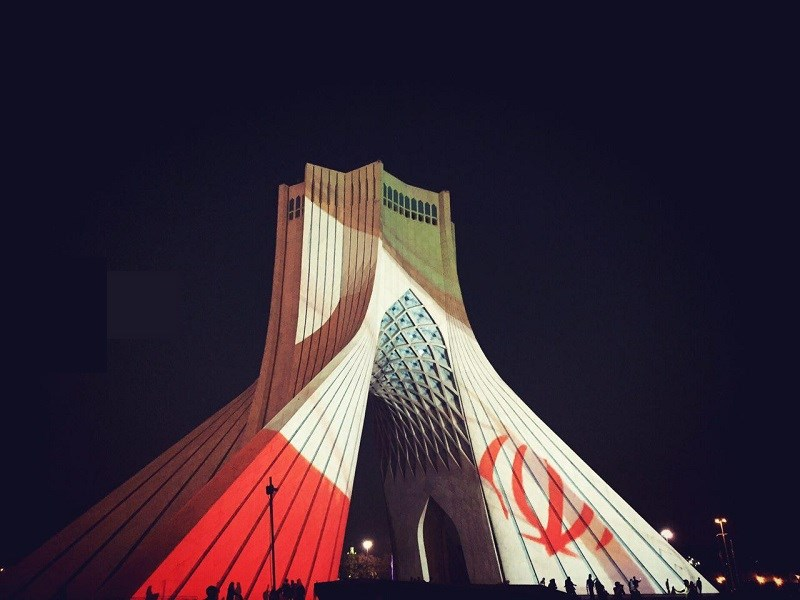
\includegraphics[width=5cm]{Picture1.png}
%	\caption{
%		تصویری از میدان آزادی
%	} 
%\end{figure}
%%%%%%%%%%%%%
%\begin{figure}[H] 
%	\centering
%	\includegraphics[height=5cm, width=5cm, angle=30]
%	{Picture1.png}
%	\caption{
%		تصویری از میدان آزادی
%	} \label{Picture1}
%\end{figure}
%%%%%%%%%%%%%
%\begin{figure}[H]  \centering
%	\subfigure[تصویر اول ]{ 		
%		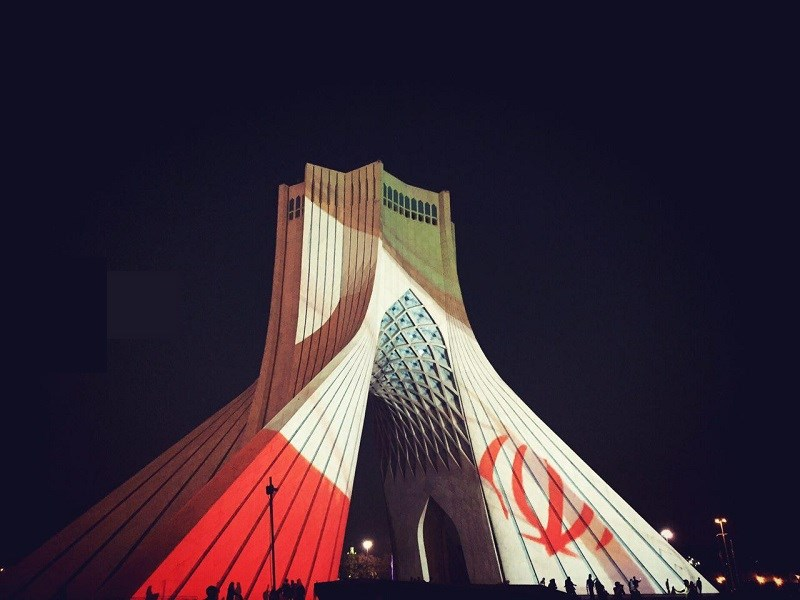
\includegraphics[width=5cm]{Picture1.png} \label{Picture1}}
%	\hspace{20mm}
%	\subfigure[تصویر دوم ]{ 	
%		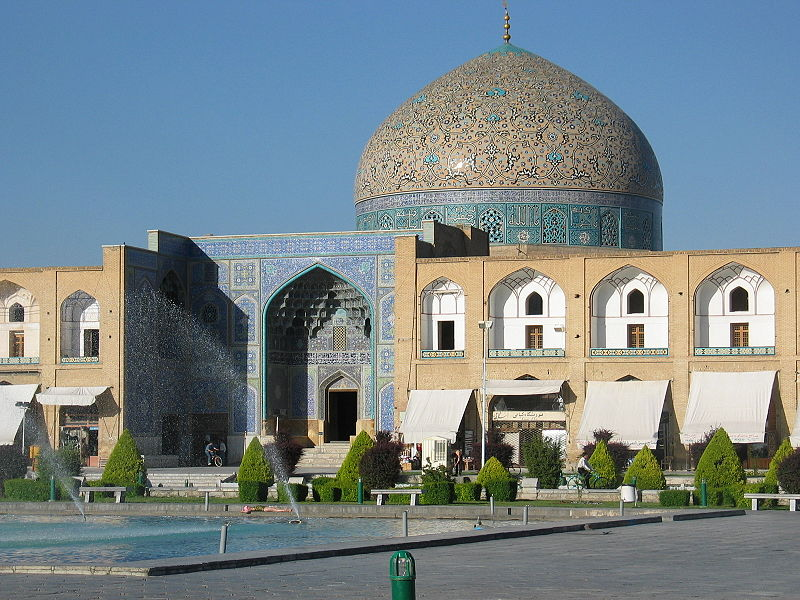
\includegraphics[width=5cm]{Picture2.png} \label{Picture2}}
%	\subfigure[تصویر سوم ]{
%		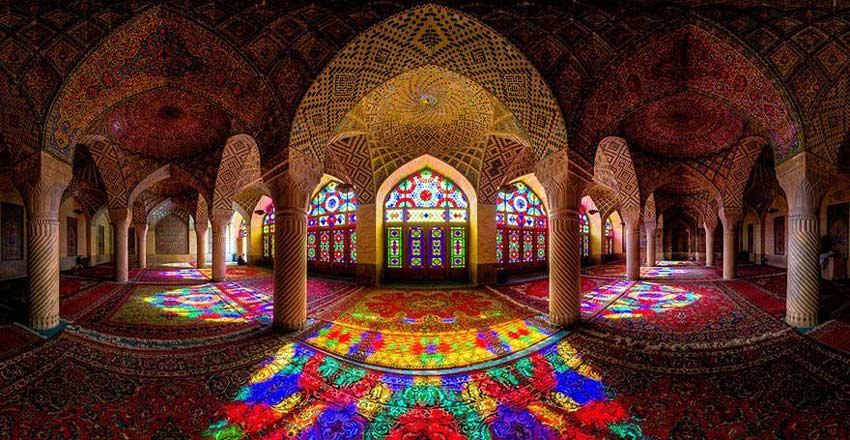
\includegraphics[width=5cm]{Picture3.png} \label{Picture1}}
%	\hspace{20mm}
%	\subfigure[تصویر چهارم]{
%		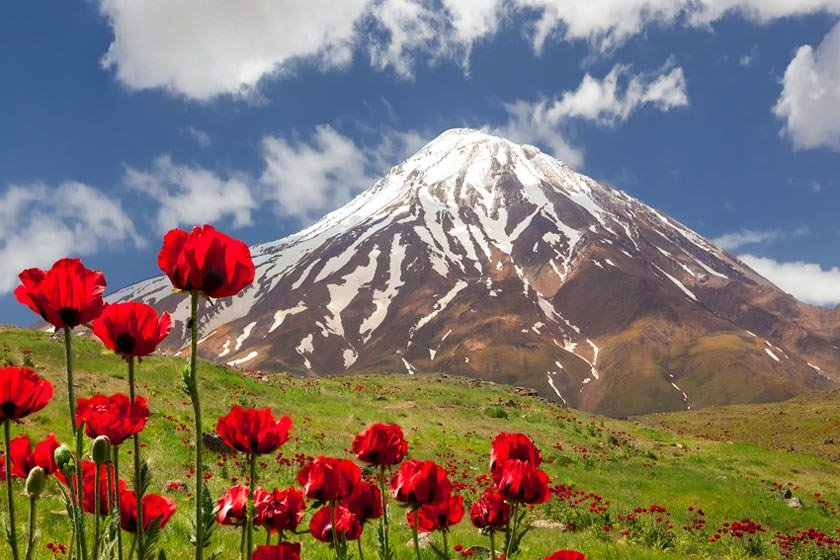
\includegraphics[width=5cm]{Picture4.png} \label{Picture2}}
%	\caption{
%		\subref{Picture1} میدان آزادی، 
%		\subref{Picture2} مسجد شیخ لطف‌الله،
%		\subref{Picture1} مسجد نصیرالملک، 
%		\subref{Picture2} کوه دماوند}\label{Pictures}
%\end{figure}

%%%%%%%%%%%%%%%%%%%%%%%%%%%%%%%%%%%%%%

%\section{جدول}
%‌\\
%\begin{table}[H]
%	\begin{center}
%		\begin{tabular}[H]{|c|c|p{4cm}|c||}
%			\hline
%			خانه11 & خانه12 &خانه13&خانه14\\
%			\hline	
%			\hline
%			\multicolumn{2}{|c|}{ادغام خانه21 و خانه22} & خانه23 & خانه24\\
%			\cline{2-3}
%			خانه31 & خانه32 &خانه33&خانه34\\
%			\hline		
%			خانه41 & خانه42 &خانه43&خانه44\\
%			\hline	
%		\end{tabular}
%	\end{center} 
%	\caption{کپشن جدول شماره‌ی یک}\label{Table1}
%\end{table}
%%%%%%%%%%%%
%% \usepackage{multirow}
%\begin{table}[]
%	\begin{center}
%		\begin{tabular}{|c|c|c|}
%			\hline
%			نشان متغیر & توضیح                            & واحد              \\ \hline
%			$F_T$      & \multicolumn{2}{c|}{\multirow{2}{*}{نیروی کشش قطار}} \\ \cline{1-1}
%			$F_D$      & \multicolumn{2}{c|}{}                                \\ \hline
%			$x$        & جابجایی قطار از مبدأ             & $m$               \\ \hline
%			$v$        & سرعت قطار                        & $m/s$             \\ \hline
%		\end{tabular}
%	\end{center} 
%\end{table}

%%%%%%%%%%%%%%%%%%%%%%%%%%%%%%%%%%%%%%
%
%\section{فرمول‌نویسی}
%‌\\
%\begin{equation}
%\left(\begin{array}{l}
%Q_{1} \\
%Q_{2}
%\end{array}\right) \equiv\left(\begin{array}{ll}
%C_{11} & C_{12} \\
%C_{21} & C_{22}
%\end{array}\right)\left(\begin{array}{l}
%V_{1} \\
%V_{2}
%\end{array}\right)
%\end{equation}
%جواب نهایی به‌صورت معادله‌ی 
%$x+1=0$ 
%خواهد بود.
%‌\\
%%%%%%%%%%%%%%%%%%%%%%
%\usepackage{amsmath}


%\begin{equation}\label{www}
%\lim_{x \to 1}
%\end{equation}


%\begin{equation} \label{eq1}
%x^{i+1} \times \sqrt[3]{y-2},\quad x_{i+1} = \frac{n+1}{n}, \quad \binom{n}{m}=\frac{n!}{m!(n-m)!}, \quad \boldsymbol{\varphi}, \quad \phi \varphi \epsilon \varepsilon, \qquad \mathbf{x}=(x_1,x_2,x_3)
%\end{equation}
%\begin{equation} \label{eq2}
%\sqrt{\frac1k \log_b x} = \sqrt{\tfrac1k \log_b x}
%\end{equation}
%\begin{equation}
%\bar{x}yz
%\left(\frac{x}{\text{متن}}\right)
%\end{equation}
%	%%%%%%%%%%%%%%%%%%%%%
%\begin{equation}
%\begin{bmatrix}
%1&2&3\\
%4&5&6\\
%7&8&9
%\end{bmatrix} 
%\end{equation}
%%%%%%%%%%%%%%%%%%%%%%
%\begin{equation}
%\begin{bmatrix}
%	
%	1 & 0 & \cdots & 0\\
%	
%	1 & 0 & \cdots & 0\\
%	
%	\vdots & \vdots & \ddots & \vdots \\
%	
%	1 & 0 & 0 & 0
%	
%\end{bmatrix}
%\end{equation}
%%%%%%%%%%%%%%%%%%%%%%
%\begin{equation}
%\left[\begin{array}{ll}
%1 & 0 \\
%1 & 0
%\end{array}\right]
%\end{equation}


%%%%%%%%%%%%%%%%%%%%%%%%%%%%%%%%%%%%%%

%\section{ارجاع‌دادن‌}\label{sec1.1}
%\subsection{ارجاع1}\label{subsec1.1}
%\subsubsection{ارجاع2}\label{subsubsec1.1}
%
%‌\\
%در
%\autoref{chap1}
%مشاهده می‌کنید. در
%\autoref{sec1.1}
%مشاهده می‌کنید. در
%\autoref{subsec1.1}
%مشاهده می‌کنید. در
%\autoref{subsubsec1.1}
%مشاهده می‌کنید. در قسمت
%\ref{sec1.1}
%مشاهده می‌کنید. در
%\nameref{sec1.1}
%مشاهده می‌کنید.
%در
%\autoref{Picture1}
%مشاهده می‌کنید.
%در
%\autoref{Picture1}
%مشاهده می‌کنید. در 
%\autoref{Table1}
%مشاهده می‌کنید. در 
%\autoref{eq1}
%مشاهده می‌کنید.
%\begin{figure}[H]
%	\centering
%	\includegraphics[height=5cm, width=5cm, angle=30]
%	{Picture1.png}
%	\caption{
%		تصویری از میدان آزادی
%	} \label{Picture1}
%\end{figure}
%
%\begin{table}[H]
%	\begin{center}
%		\begin{tabular}[H]{|c|c|p{4cm}|c||}
%			\hline
%			خانه11 & خانه12 &خانه13&خانه14\\
%			\hline	
%			\hline
%			\multicolumn{2}{|c|}{ادغام خانه21 و خانه22} & خانه23 & خانه24\\
%			\cline{2-3}
%			خانه31 & خانه32 &خانه33&خانه34\\
%			\hline		
%			خانه41 & خانه42 &خانه43&خانه44\\
%			\hline	
%		\end{tabular}
%	\end{center} 
%	\caption{کپشن جدول شماره‌ی یک}\label{Table1}
%\end{table}
%
%%\usepackage{amsmath}
%
%\begin{equation} \label{eq1}
%x^{i+1} \times \sqrt[3]{y-2},\quad x_{i+1} = \tfrac12\frac{n+1}{n}, \quad \binom{n}{m}=\frac{n!}{m!(n-m)!}, \quad \boldsymbol{\varphi}, \quad \phi \varphi \epsilon \varepsilon, \qquad \mathbf{x}=(x_1,x_2,x_3)
%\end{equation}
%
%
%
%برای مطالعه‌ی ادامه‌ی قضایا به 
%\cite{bidabad2007classification}
%مراجعه فرمایید \cite{aa}.
%










	\chapter{سوالات شبیه‌سازی}
\section{پاسخ سوال اول (\lr{Problem 9.4-1})}
در حالت کلی برای سیستم داریم:



	%\include{chapter3}
	%\include{chapter4}
	%\include{chapter5}
	
	%--------------------------------------------------------------------------appendix( مراجع و پیوست ها)
	\chapterfont{\vspace*{-2em}\centering\LARGE}%
	
	\appendix

	\bibliographystyle{plain-fa}
	\bibliography{references}

	\chapter*{‌پیوست}
\markboth{پیوست}{}
\addcontentsline{toc}{chapter}{پیوست}
موضوعات مرتبط با متن گزارش پایان نامه كه در يكی از گروه‌های زير قرار می‌گيرد، در بخش پيوست‌ها آورده شوند:
\begin{enumerate}
\item  اثبات های رياضی يا عمليات رياضی طولانی‌.‌
\item داده و اطلاعات نمونه (های) مورد مطالعه (\lr{Case Study}) چنانچه طولانی باشد‌.‌
\item نتايج كارهای ديگران چنانچه نياز به تفصيل باشد‌.‌
\item مجموعه تعاريف متغيرها و پارامترها، چنانچه طولانی بوده و در متن به انجام نرسيده باشد‌.‌
\end{enumerate}
% براي شماره‌گذاري روابط، جداول و اشكال موجود در پيوست‌ از ساختار متفاوتي نسبت به متن اصلي استفاده مي‌شود كه در زير به‌عنوان نمونه نمايش داده شده‌است. 
% \begin{equation}
%F=ma
%\end{equation}
\section*{کد میپل }
‌\\
\begin{latin}
\begin{verbatim}

with(DifferentialGeometry):
with(Tensor):
DGsetup([x, y, z], M)
																	frame name: M
a := evalDG(D_x)
																	D_x
b := evalDG(-2 y z D_x+2 x D_y/z^3-D_z/z^2)


\end{verbatim}
\end{latin}
\section*{کد متلب }
‌\\
\begin{latin}
	\lstinputlisting[language=Matlab, frame=single]{System_ctrb.m}
\end{latin}
‌\\
\begin{latin}
	\begin{lstlisting}[language=C]
	#include <stdio.h>
	#define N 10
	/* Block
	* comment */
	
	int main()
	{
	int i;
	
	// Line comment.
	puts("Hello world!");
	
	for (i = 0; i < N; i++)
	{
	puts("LaTeX is also great for programmers!");
	}
	
	return 0;
	}
	\end{lstlisting}
\end{latin}
‌\\
\begin{latin}
	\begin{lstlisting}[mathescape=true]
	// calculate  $a_{ij}$
	$a_{ij} = a_{jj}/a_{ij} + \alpha$;
	\end{lstlisting}
\end{latin}
	%--------------------------------------------------------------------------dictionary(واژه نامه ها)
	%اگر مایل به داشتن صفحه واژه‌نامه نیستید، خط زیر را غیر فعال کنید.
	\parindent=0pt
	%
\chapter*{واژه‌نامه‌ی فارسی به انگلیسی}
\pagestyle{style9}

\addcontentsline{toc}{chapter}{واژه‌نامه‌ی فارسی به انگلیسی}
%%%%%%
\begin{multicols*}{2}

{\bf آ}
\vspace*{3mm}


\farsiTOenglish{اسکالر}{Scalar}


\vspace*{3mm}
{\bf ب}
\vspace*{3mm}

\farsiTOenglish{بالابر}{Lift}


\vspace*{3mm}
{\bf پ}
%%\vspace*{3mm}

\farsiTOenglish{پایا}{Invariant}



\vspace*{3mm}
{\bf ت}
%%\vspace*{3mm}

\farsiTOenglish{ تناظر }{Correspondence}


\vspace*{3mm}
{\bf ث}
%%\vspace*{3mm}

\farsiTOenglish{ثابت‌ساز}{Stabilizer}

\vspace*{3mm}
{\bf ج}
%%\vspace*{3mm}

\farsiTOenglish{جایگشت}{Permutation}



\vspace*{3mm}
{\bf چ}
%%\vspace*{3mm}


\farsiTOenglish{چند جمله‌ای }{Polynomial}

\vspace*{3mm}
{\bf ح}
%%\vspace*{3mm}

\farsiTOenglish{حاصل‌ضرب دکارتی}{Cartesian product}


\vspace*{3mm}
{\bf خ}
%%\vspace*{3mm}

\farsiTOenglish{خودریختی}{Automorphism}

\vspace*{3mm}
{\bf د}
%%\vspace*{3mm}

\farsiTOenglish{درجه}{Degree}


\vspace*{3mm}
{\bf ر}
%%\vspace*{3mm}


\farsiTOenglish{ریزپردازنده}{microprocessor}


\vspace*{3mm}
{\bf ز}
%%\vspace*{3mm}


\farsiTOenglish{زیرمدول}{Submodule}


\vspace*{3mm}
{\bf س}
%%\vspace*{3mm}

\farsiTOenglish{سرشت}{Character}


\vspace*{3mm}
{\bf ص}
%%\vspace*{3mm}

\farsiTOenglish{صادقانه}{Faithful}

\vspace*{3mm}
{\bf ض}
%%\vspace*{3mm}

\farsiTOenglish{ضرب داخلی}{Inner product}

\vspace*{3mm}
{\bf ط}
%%\vspace*{3mm}


\farsiTOenglish{طوقه}{Loop}


\vspace*{3mm}
{\bf ظ}
%%\vspace*{3mm}


\farsiTOenglish{ظرفیت}{Valency}
 
\vspace*{3mm}
{\bf ع}
%%\vspace*{3mm}


\farsiTOenglish{عدم مجاورت}{Nonadjacency}



\vspace*{3mm}
{\bf ف}
%%\vspace*{3mm}

\farsiTOenglish{فضای برداری}{Vector space}



\vspace*{3mm}
{\bf ک}
%%\vspace*{3mm}

\farsiTOenglish{کاملاً تحویل‌پذیر}{Complete reducibility}


\vspace*{3mm}
{\bf گ}
%%\vspace*{3mm}


\farsiTOenglish{گراف}{Graph}



\vspace*{3mm}
{\bf م}
%%\vspace*{3mm}

\farsiTOenglish{ماتریس جایگشتی}{Permutation matrix }


\vspace*{3mm}
{\bf ن}
%%\vspace*{3mm}

\farsiTOenglish{ناهمبند}{Disconnected}


\vspace*{3mm}
{\bf و}
%%\vspace*{3mm}

\farsiTOenglish{وارون‌پذیر}{Invertible}


\vspace*{3mm}
{\bf ه}
%%\vspace*{3mm}

\farsiTOenglish{همبند}{Connected}



\vspace*{3mm}
{\bf ی}
%%\vspace*{3mm}

\farsiTOenglish{یال}{Edge}




\end{multicols*}%
	%%%%%%
\chapter*{ واژه‌نامه‌ی انگلیسی به فارسی}
\pagestyle{style9}
\lhead{\thepage}\rhead{واژه‌نامه‌ی انگلیسی به فارسی}
\addcontentsline{toc}{chapter}{واژه‌نامه‌ی انگلیسی به فارسی}

\LTRmulticolcolumns
\begin{multicols}{2}
{\hfill\bf  \lr{A}}
%%\vspace*{1.5mm}

\englishTOfarsi{Automorphism}{خودریختی}

\vspace*{3mm}
{\hfill\bf   \lr{B}}
%%\vspace*{1.5mm}

\englishTOfarsi{Bijection}{دوسویی}

\vspace*{3mm}
{\hfill\bf   \lr{C}}
%%\vspace*{1.5mm}

\englishTOfarsi{Cycle group}{گروه دوری}

\vspace*{3mm}
{\hfill\bf   \lr{D}}
%%\vspace*{1.5mm}

\englishTOfarsi{Degree}{درجه}

\vspace*{3mm}
{\hfill\bf   \lr{E}}
%%\vspace*{1.5mm}

\englishTOfarsi{Edge}{یال}

\vspace*{3mm}
{\hfill\bf   \lr{F}}
%%\vspace*{1.5mm}

\englishTOfarsi{Function}{تابع}

\vspace*{3mm}
{\hfill\bf   \lr{G}}
%%\vspace*{1.5mm}

\englishTOfarsi{Group}{گروه}

\vspace*{3mm}
{\hfill\bf   \lr{H}}
%%\vspace*{1.5mm}

\englishTOfarsi{Homomorphism}{همریختی}

\vspace*{3mm}
{\hfill\bf   \lr{I}}
%%\vspace*{1.5mm}

\englishTOfarsi{Invariant}{پایا}

\vspace*{3mm}
{\hfill\bf   \lr{L}}
%%\vspace*{1.5mm}

\englishTOfarsi{Lift}{بالابر}

\vspace*{3mm}
{\hfill\bf   \lr{M}}
%%\vspace*{1.5mm}

\englishTOfarsi{Module}{مدول}

\vspace*{3mm}
{\hfill\bf   \lr{N}}
%%\vspace*{1.5mm}

\englishTOfarsi{Natural map}{نگاشت طبیعی}

\vspace*{3mm}
{\hfill\bf   \lr{O}}
%%\vspace*{1.5mm}

\englishTOfarsi{One to One}{یک به یک}

\vspace*{3mm}
{\hfill\bf   \lr{P}}
%%\vspace*{1.5mm}

\englishTOfarsi{Permutation group}{گروه جایگشتی}

\vspace*{3mm}
{\hfill\bf   \lr{Q}}
%%\vspace*{1.5mm}

\englishTOfarsi{Quotient graph}{گراف خارج‌قسمتی}

 \vspace*{3mm}
{\hfill\bf   \lr{R}}
%%\vspace*{1.5mm}

\englishTOfarsi{Reducible}{تحویل پذیر}

\vspace*{3mm}
{\hfill\bf   \lr{S}}
%%\vspace*{1.5mm}

\englishTOfarsi{Sequence}{دنباله}

 \vspace*{3mm}
{\hfill\bf   \lr{T}}
%%\vspace*{1.5mm}

\englishTOfarsi{Trivial character}{سرشت بدیهی}

\vspace*{3mm}
{\hfill\bf   \lr{U}}
%%\vspace*{1.5mm}

\englishTOfarsi{Unique}{منحصربفرد}

\vspace*{3mm}
{\hfill\bf   \lr{V}}
%%\vspace*{1.5mm}

\englishTOfarsi{Vector space}{فضای برداری}
\end{multicols}
	%--------------------------------------------------------------------------index(نمایه)
	%اگر مایل به داشتن صفحه نمایه نیستید، خط زیر را غیر فعال کنید.
	\pagestyle{style7}
	\printindex
	\pagestyle{style7}
	
	\end{document}